\documentclass[11pt,a4paper]{article}
\usepackage[utf8]{inputenc}
\usepackage[T1]{fontenc}
\usepackage[brazil]{babel}
\usepackage{lmodern}
\usepackage[margin=2.3cm]{geometry}
\usepackage{amsmath, amssymb, amsthm}
\usepackage{booktabs}
\usepackage{array}
\usepackage{tabularx}
\usepackage{graphicx}
\usepackage{xcolor}
\usepackage{inconsolata}
\usepackage{listings}
\usepackage[most]{tcolorbox}
\usepackage{enumitem}
\usepackage{fancyhdr}
\usepackage{hyperref}
\usepackage[backend=bibtex, style=numeric, sorting=none]{biblatex}
\addbibresource{3-reference/ref.bib}

% ============================================================
% CORES, ESTILOS DE CÓDIGO E CAIXAS TEÓRICAS
% ============================================================
\definecolor{primary}{RGB}{26, 115, 232}
\definecolor{darkred}{RGB}{178, 34, 34}
\definecolor{accent}{RGB}{46, 125, 50}
\definecolor{backcolour}{rgb}{0.96,0.96,0.94}
\definecolor{codegreen}{rgb}{0,0.55,0}
\definecolor{codegray}{rgb}{0.45,0.45,0.45}
\definecolor{codepurple}{rgb}{0.58,0,0.82}

\lstdefinestyle{pythonstyle}{
    backgroundcolor=\color{backcolour},
    commentstyle=\color{codegreen}\itshape,
    keywordstyle=\color{primary}\bfseries,
    numberstyle=\tiny\color{codegray},
    stringstyle=\color{codepurple},
    basicstyle=\ttfamily\footnotesize,
    breakatwhitespace=false,
    breaklines=true,
    captionpos=b,
    keepspaces=true,
    numbers=left,
    numbersep=5pt,
    showspaces=false,
    showstringspaces=false,
    showtabs=false,
    tabsize=2,
    language=Python,
    extendedchars=true,
    morekeywords={as, True, False, None, np, linspace, exp, sum, abs, sqrt, ceil}
}
\lstset{style=pythonstyle}

\hypersetup{
    colorlinks=true,
    linkcolor=darkred,
    urlcolor=primary,
    citecolor=accent,
    pdftitle={Material Técnico Completo: Integração Numérica e Método dos Trapézios},
    pdfauthor={Prof. João Cardoso}
}

\pagestyle{fancy}
\fancyhf{}
\fancyhead[L]{\small \textcolor{darkred}{\textbf{Material Técnico --- Integração Numérica}}}
\fancyhead[R]{\small \textcolor{gray}{Prof. João Cardoso}}
\fancyfoot[C]{\small \thepage}
\renewcommand{\headrulewidth}{0.4pt}

\newtheorem{teorema}{Teorema}[section]
\newtheorem{proposicao}{Proposição}[section]
\newtheorem{observacao}{Observação}[section]

\newtcolorbox{teobox}[1]{
    colback=white,
    colframe=darkred,
    fonttitle=\bfseries,
    title=#1,
    arc=2mm,
    boxrule=0.9pt,
    breakable
}

\newtcolorbox{codigobox}[1]{
    colback=backcolour,
    colframe=primary,
    fonttitle=\bfseries\small,
    title=#1,
    arc=2mm,
    boxrule=0.8pt,
    breakable
}

\begin{document}

% ============================================================
% CAPA / CABEÇALHO TÉCNICO
% ============================================================
\begin{titlepage}
    \centering
    \vspace*{1.5cm}
    {\large \textsc{Disciplina de Cálculo Numérico / Métodos Numéricos}}\\[1.2cm]
    {\Huge \bfseries \textcolor{darkred}{Integração Numérica}}\\[0.5cm]
    {\LARGE \bfseries Das Fórmulas de Newton-Cotes ao Método dos Trapézios: Teoria, Análise de Erro e Computação Científica em Python}\\[1.4cm]
    \rule{0.75\textwidth}{1.5pt}\\[0.8cm]
    {\large \textbf{Material Técnico Completo de Apoio e Conferência Pós-Aula}}\\[0.4cm]
    {\large \textbf{Autor:} Prof. João Cardoso}\\[1.2cm]
    \begin{tcolorbox}[colback=backcolour, colframe=primary, width=0.88\textwidth, arc=2mm]
        \small
        \textbf{Resumo Técnico:} Este documento apresenta a fundamentação matemática, computacional e aplicada da Quadratura Numérica, conectando a recapitulação das Fórmulas Fechadas de Newton-Cotes ao estudo detalhado do Método dos Trapézios (simples e composto). Inclui dedução integral dos coeficientes de Cotes, demonstração rigorosa do erro de truncamento via Teorema do Valor Médio Ponderado para Integrais, expansão assintótica de Euler-Maclaurin, análise da interação com erros de arredondamento IEEE 754, quatro exercícios resolvidos completos, códigos-fonte vetorizados em Python, visualizações gráficas, links para animações em vídeo e preparação formal para os Métodos de Simpson ($1/3$ e $3/8$).\\[0.4em]
        \textbf{Repositório Oficial (Códigos, Gráficos e Vídeos):}\\
        \href{https://github.com/Zuluke/numerical-calculus.git}{\nolinkurl{https://github.com/Zuluke/numerical-calculus.git}}
    \end{tcolorbox}
    \vfill
    {\normalsize \today}
\end{titlepage}

\tableofcontents
\newpage

% ============================================================
% SEÇÃO 1: INTRODUÇÃO E MOTIVAÇÃO
% ============================================================
\section{Introdução e Motivação da Integração Numérica}

No Cálculo Diferencial e Integral clássico, o cálculo de uma integral definida
\begin{equation}
    I(f) = \int_{a}^{b} f(x)\,dx
\end{equation}
baseia-se no \textbf{Teorema Fundamental do Cálculo (TFC)}: se $f$ é contínua em $[a, b]$ e possui uma primitiva (antiderivada) conhecida $F(x)$ tal que $F'(x) = f(x)$, então $I(f) = F(b) - F(a)$. Embora elegante, o método analítico encontra barreiras severas em problemas reais da Engenharia, Física, Estatística e Ciência da Computação \cite{santos2010, ruggiero1996, burden2016, mesquita2026}.

\subsection{As Duas Situações Fundamentais}
A necessidade da \emph{Quadratura Numérica} (ou Integração Numérica) emerge tipicamente em dois cenários inevitáveis:
\begin{enumerate}[leftmargin=1.6em]
    \item \textbf{Função Desconhecida Analiticamente (Dados Experimentais ou Tabulados)}: Em aplicações empíricas, não dispomos de uma expressão fechada para $f(x)$, mas sim de uma tabela discreta de pontos $\{(x_i, y_i)\}_{i=0}^n$ onde $y_i = f(x_i)$ foi coletado por sensores, medidores de vazão, velocímetros ou ensaios laboratoriais.
    \item \textbf{Função Conhecida sem Primitiva Elementar ou Algebricamente Proibitiva}: Mesmo quando $f(x)$ possui fórmula analítica simples, o Teorema de Liouville demonstra que diversas funções elementares não admitem primitiva expressável como combinação finita de funções elementares. Exemplos clássicos incluem:
    \begin{itemize}
        \item A \emph{Integral Gaussiana} (base da Distribuição Normal em Estatística): $\int_a^b e^{-x^2}\,dx$;
        \item O \emph{Seno Integral} (processamento de sinais e ótica): $\operatorname{Si}(x) = \int_0^x \frac{\sin t}{t}\,dt$;
        \item As \emph{Integrais Elípticas} (comprimento de arco de elipses e período real de pêndulos): $\int_a^b \sqrt{1 - k^2 \sin^2 \theta}\,d\theta$;
        \item Integrais de funções altamente complexas obtidas por simbologia automática onde a antiderivada é instável ou excessivamente dispendiosa.
    \end{itemize}
\end{enumerate}

\subsection{Aplicações Práticas na Engenharia e Ciência de Dados}
\begin{itemize}[leftmargin=1.5em]
    \item \textbf{Mecânica e Termodinâmica}: Determinação do trabalho mecânico $W = \int_{x_0}^{x_1} F(x)\,dx$ a partir de curvas experimentais força $\times$ deslocamento, ou energia transferida por potência variável $E = \int_{t_0}^{t_1} P(t)\,dt$.
    \item \textbf{Hidrologia e Engenharia Civil}: Cálculo de vazão total escoada em rios por meio de perfis discretos de velocidade em seções transversais, ou volumes de terraplenagem.
    \item \textbf{Aprendizado de Máquina (Machine Learning)}: Cálculo da área sob a curva ROC (\emph{Area Under the Curve} --- \textbf{AUC-ROC}), utilizada para avaliar classificadores binários a partir de pares discretos $(\text{FPR}_i, \text{TPR}_i)$ variando limiares de decisão, implementado nativamente pela regra dos trapézios no \texttt{scikit-learn} e no \texttt{SciPy} \cite{scipy_trapezoid, chapra2016}.
\end{itemize}

% ============================================================
% SEÇÃO 2: RECAPITULAÇÃO DAS FÓRMULAS DE NEWTON-COTES
% ============================================================
\section{Recapitulação: O Guarda-Chuva das Fórmulas de Newton-Cotes}

A filosofia central das \textbf{Fórmulas de Newton-Cotes} consiste em substituir o integrando complexo ou tabulado $f(x)$ por um polinômio interpolador $P_n(x)$ de grau no máximo $n$, cuja integração é trivial, exata e linear nos valores nodais \cite{santos2010, claudio1994, mesquita2026}.

\subsection{Formulação Geral via Polinômio de Lagrange}
Considere o intervalo $[a, b]$ particionado em $n$ subintervalos idênticos de largura (passo)
\begin{equation}
    h = \frac{b - a}{n}, \qquad x_k = x_0 + k h \quad (k = 0, 1, \dots, n), \quad x_0 = a,\; x_n = b.
\end{equation}
Utilizando a forma de Lagrange, $f(x) = P_n(x) + R_n(x)$, onde
\begin{equation}
    P_n(x) = \sum_{k=0}^{n} L_k^n(x) f(x_k), \qquad L_k^n(x) = \prod_{\substack{j=0 \\ j \neq k}}^{n} \frac{x - x_j}{x_k - x_j}.
\end{equation}
Integrando ambos os membros entre $x_0$ e $x_n$ e usando a linearidade da integral:
\begin{equation}
    \int_{x_0}^{x_n} f(x)\,dx = \sum_{k=0}^{n} \left( \int_{x_0}^{x_n} L_k^n(x)\,dx \right) f(x_k) + \int_{x_0}^{x_n} R_n(x)\,dx = \sum_{k=0}^{n} C_k^n f(x_k) + T,
\end{equation}
em que os coeficientes $C_k^n = \int_{x_0}^{x_n} L_k^n(x)\,dx$ são chamados \textbf{Coeficientes (ou Pesos) de Cotes} e $T = \int_{x_0}^{x_n} R_n(x)\,dx$ é o \textbf{Erro de Truncamento}.

\subsection{Dedução dos Coeficientes $C_k^n$ por Mudança de Variável}
Introduzindo a variável adimensional $z = \frac{x - x_0}{h}$ (portanto $x = x_0 + z h$ e $dx = h\,dz$), os limites $x = x_0$ e $x = x_n$ mapeiam-se em $z = 0$ e $z = n$. Ademais, para cada índice $j \neq k$:
\[
\frac{x - x_j}{x_k - x_j} = \frac{(x_0 + z h) - (x_0 + j h)}{(x_0 + k h) - (x_0 + j h)} = \frac{z - j}{k - j}.
\]
Substituindo no integrando:
\[
C_k^n = h \int_0^n \prod_{\substack{j=0 \\ j \neq k}}^{n} \frac{z - j}{k - j}\,dz = \frac{h}{\prod_{j \neq k} (k - j)} \int_0^n \frac{\pi_n(z)}{z - k}\,dz, \quad \text{com } \pi_n(z) = \prod_{j=0}^{n} (z - j).
\]
Observando que o denominador fatora-se em termos de fatoriais com sinal alternado:
\[
\prod_{\substack{j=0 \\ j \neq k}}^{n} (k - j) = \underbrace{k(k-1)\cdots 1}_{k!} \cdot \underbrace{(-1)(-2)\cdots (-(n-k))}_{(-1)^{n-k}(n-k)!} = (-1)^{n-k} k!(n - k)!,
\]
obtemos a \textbf{Fórmula Geral dos Coeficientes Fechados de Newton-Cotes}:
\begin{equation}
    C_k^n = \frac{(-1)^{n-k}\,h}{k!(n - k)!} \int_0^n \frac{\pi_n(z)}{z - k}\,dz, \qquad k = 0, 1, \dots, n.
\end{equation}
Notavelmente, os coeficientes $C_k^n / h$ dependem \textbf{exclusivamente} do grau $n$ e do índice $k$, sendo totalmente independentes da função $f$ e dos limites particulares $a$ e $b$.

\subsection{Hierarquia das Regras Fechadas e Fenômeno de Runge}
A Tabela~\ref{tab:newton_cotes} sintetiza os primeiros membros da família fechada de Newton-Cotes \cite{burden2016, chapra2016}.

\begin{table}[h!]
\centering
\caption{Primeiras Fórmulas Fechadas de Newton-Cotes (sem subdivisão composta).}
\label{tab:newton_cotes}
\small
\begin{tabular}{clccc}
\toprule
\textbf{Grau ($n$)} & \textbf{Nome Clássico} & \textbf{Fórmula de Quadratura} & \textbf{Grau de Precisão} & \textbf{Erro ($T$)} \\
\midrule
$n = 1$ & \textbf{Regra do Trapézio} & $\frac{h}{2}\big[f(x_0) + f(x_1)\big]$ & $1$ & $-\frac{h^3}{12} f''(\xi)$ \\
$n = 2$ & Regra $1/3$ de Simpson & $\frac{h}{3}\big[f(x_0) + 4f(x_1) + f(x_2)\big]$ & $3$ & $-\frac{h^5}{90} f^{(4)}(\xi)$ \\
$n = 3$ & Regra $3/8$ de Simpson & $\frac{3h}{8}\big[f(x_0) + 3f(x_1) + 3f(x_2) + f(x_3)\big]$ & $3$ & $-\frac{3h^5}{80} f^{(4)}(\xi)$ \\
$n = 4$ & Regra de Boole & $\frac{2h}{45}\big[7f_0 + 32f_1 + 12f_2 + 32f_3 + 7f_4\big]$ & $5$ & $-\frac{8h^7}{945} f^{(6)}(\xi)$ \\
\bottomrule
\end{tabular}
\end{table}

\begin{observacao}[Por que não usar $n$ elevado em um único polinômio global?]
Poderia parecer natural elevar $n$ indefinidamente ($n = 10, 20, \dots$) em $[a, b]$ para melhorar a precisão. Todavia, dois fenômenos matemáticos severos inviabilizam essa abordagem \cite{ruggiero1996, burden2016}:
\begin{enumerate}
    \item \textbf{Fenômeno de Runge}: A interpolação polinomial global em nós equidistantes não converge necessariamente para $f(x)$ quando $n \to \infty$ (caso célebre: $f(x) = \frac{1}{1 + 25x^2}$ em $[-1, 1]$), apresentando oscilações violentas junto às extremidades.
    \item \textbf{Pesos Negativos e Cancelamento Catastrófico}: A partir de $n = 8$ (e para todo $n \ge 10$), surgem coeficientes de Cotes \textbf{estritamente negativos} ($C_k^n < 0$). Em aritmética de ponto flutuante, somar parcelas grandes de sinais opostos amplifica erros de arredondamento e de medição experimental ($\sum |C_k^n| > b - a$).
\end{enumerate}
A solução numérica robusta consiste em \textbf{fixar o grau local baixo} ($n=1$ para Trapézios, $n=2$ para Simpson) e aplicar a regra \textbf{de forma composta} em vários subintervalos.
\end{observacao}

% ============================================================
% SEÇÃO 3: MÉTODO DOS TRAPÉZIOS (SIMPLES E COMPOSTO)
% ============================================================
\section{O Método dos Trapézios: Simples e Composto}

\subsection{Conexão Direta com Newton-Cotes ($n = 1$)}
Substituindo $n = 1$ na fórmula geral dos coeficientes de Cotes, temos $\pi_1(z) = z(z - 1)$:
\begin{align}
    C_0^1 &= \frac{(-1)^{1-0} h}{0!\,1!} \int_0^1 \frac{z(z-1)}{z-0}\,dz = -h \int_0^1 (z - 1)\,dz = -h \left[ \frac{z^2}{2} - z \right]_0^1 = \frac{h}{2}, \\
    C_1^1 &= \frac{(-1)^{1-1} h}{1!\,0!} \int_0^1 \frac{z(z-1)}{z-1}\,dz = h \int_0^1 z\,dz = h \left[ \frac{z^2}{2} \right]_0^1 = \frac{h}{2}.
\end{align}
Consequentemente, a \textbf{Regra do Trapézio Simples} sobre $[x_0, x_1]$ (com $h = x_1 - x_0$) escreve-se:
\begin{equation}
    \int_{x_0}^{x_1} f(x)\,dx = \frac{h}{2}\big[f(x_0) + f(x_1)\big] + T_1.
\end{equation}
Geometricamente, a aproximação equivale exatamente à área do trapézio retângulo de altura $h = x_1 - x_0$ e bases paralelas $f(x_0)$ e $f(x_1)$, substituindo a curva $f(x)$ pelo segmento de reta secante que liga $(x_0, f(x_0))$ a $(x_1, f(x_1))$.

\begin{figure}[h!]
    \centering
    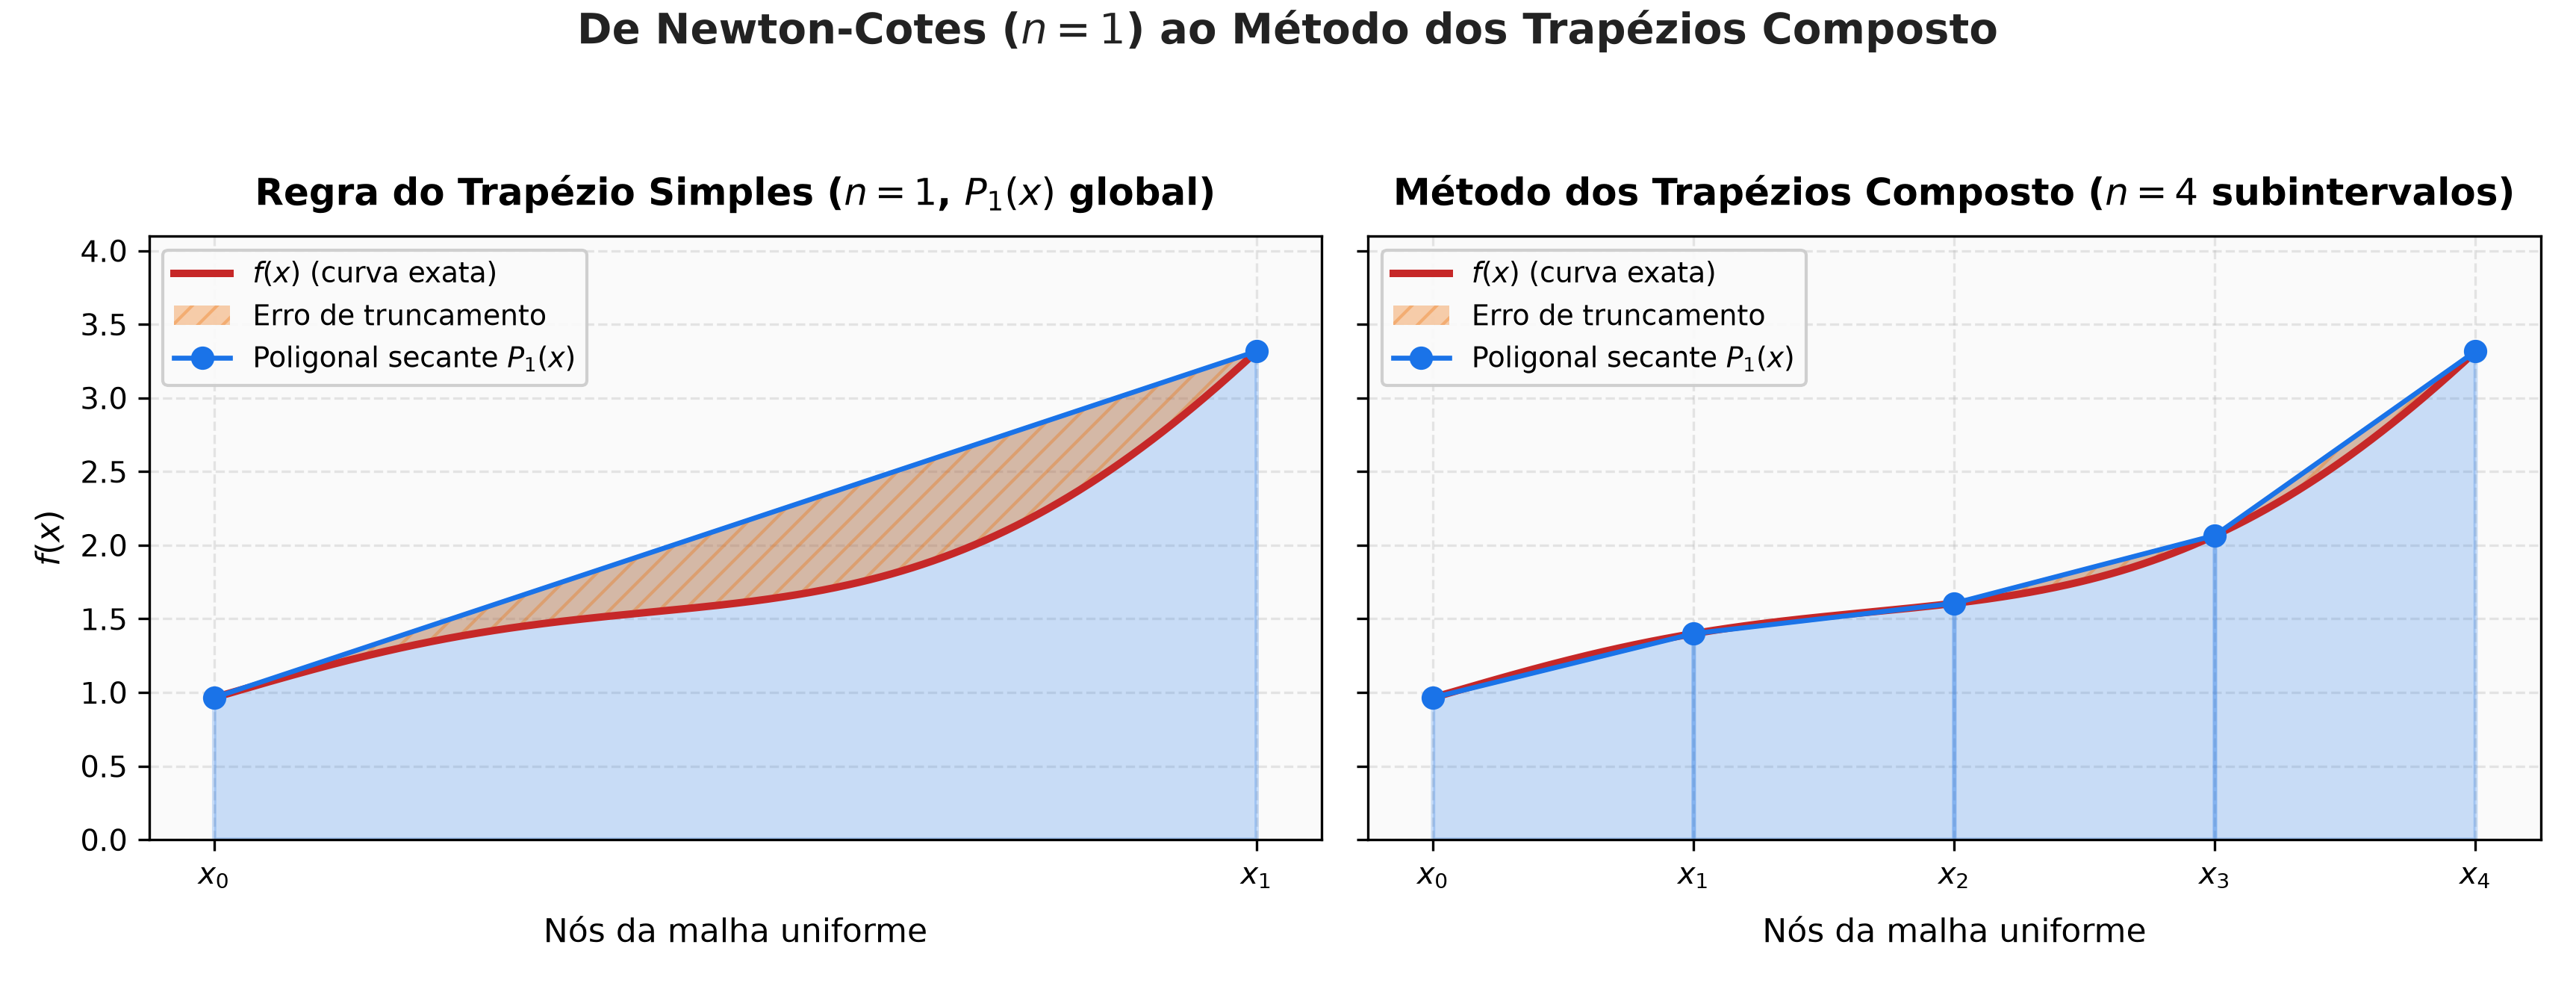
\includegraphics[width=0.95\textwidth]{images/fig_newton_cotes_trapezio.png}
    \caption{Comparação geométrica entre a Regra do Trapézio Simples ($n=1$) e o Método dos Trapézios Composto ($n=4$ subintervalos). As regiões hachuradas em laranja evidenciam a drástica redução do erro de truncamento ao refinar a malha \cite{cardoso2026_github}.}
    \label{fig:trapezio_geom}
\end{figure}

\subsection{Dedução da Fórmula Composta (Generalizada)}
Para controlar o erro sobre um intervalo amplo $[a, b]$, particionamos $[a, b]$ em $n \ge 1$ subintervalos iguais $[x_0, x_1], [x_1, x_2], \dots, [x_{n-1}, x_n]$ com passo $h = \frac{b - a}{n}$ e $n + 1$ nós $x_i = a + i h$. Pela aditividade da integral de Riemann:
\begin{align}
    \int_{a}^{b} f(x)\,dx &= \sum_{i=0}^{n-1} \int_{x_i}^{x_{i+1}} f(x)\,dx \nonumber \\
    &= \sum_{i=0}^{n-1} \left( \frac{h}{2}\big[f(x_i) + f(x_{i+1})\big] + T_{i+1} \right) \nonumber \\
    &= \frac{h}{2}\Big[ f(x_0) + 2f(x_1) + 2f(x_2) + \dots + 2f(x_{n-1}) + f(x_n) \Big] + \sum_{i=0}^{n-1} T_{i+1}.
\end{align}
Colocando $h$ em evidência, obtemos a \textbf{Fórmula Composta do Método dos Trapézios} \cite{santos2010, mesquita2026}:
\begin{equation}
    \int_{x_0}^{x_n} f(x)\,dx = h \left[ \frac{f(x_0) + f(x_n)}{2} + \sum_{i=1}^{n-1} f(x_i) \right] + T_t.
\end{equation}
Na notação didática clássica adotada em cursos de Métodos Numéricos \cite{santos2010, mesquita2026}, agrupam-se os termos em:
\begin{equation}
    I_T = h \left( \frac{E}{2} + I + P \right),
\end{equation}
onde $E = f(x_0) + f(x_n)$ representa a soma das imagens nos extremos, $I = \sum_{\substack{i=1 \\ i \text{ ímpar}}}^{n-1} f(x_i)$ a soma nos nós internos de índice ímpar e $P = \sum_{\substack{i=2 \\ i \text{ par}}}^{n-2} f(x_i)$ a soma nos nós internos de índice par (essa decomposição facilita a comparação e o reuso imediato ao estudar o Método de Simpson na aula seguinte!).

% ============================================================
% SEÇÃO 4: ANÁLISE DE ERRO E ESTABILIDADE
% ============================================================
\section{Análise Rigorosa do Erro de Truncamento e Estabilidade}

\begin{teorema}[Erro Local e Global do Método dos Trapézios]
Seja $f \in C^2([a, b])$, ou seja, contínua com derivada segunda contínua em $[a, b]$. Então, para qualquer partição uniforme em $n \ge 1$ subintervalos de largura $h = (b - a)/n$, o erro de truncamento global $T_t = \int_a^b f(x)\,dx - I_T$ satisfaz:
\begin{equation}
    T_t = -\frac{n h^3}{12} f''(\xi) = -\frac{(b - a) h^2}{12} f''(\xi) = -\frac{(b - a)^3}{12 n^2} f''(\xi), \qquad \text{para algum } \xi \in (a, b).
\end{equation}
Consequentemente, definindo $M_2 = \max_{x \in [a, b]} |f''(x)|$, vale a cota superior:
\begin{equation}
    |T_t| \le \frac{n h^3}{12} M_2 = \frac{(b - a)^3}{12 n^2} M_2.
\end{equation}
\end{teorema}

\begin{proof}
Considere um subintervalo genérico $[x_i, x_{i+1}]$ de comprimento $h$. Pelo Teorema do Erro na Interpolação Polinomial de grau $1$ \cite{burden2016, ruggiero1996}, para todo $x \in [x_i, x_{i+1}]$ existe $\eta(x) \in (x_i, x_{i+1})$ tal que:
\[
R_1(x) = f(x) - P_1(x) = \frac{f''(\eta(x))}{2!} (x - x_i)(x - x_{i+1}).
\]
Observamos que o fator quadrático $w(x) = (x - x_i)(x - x_{i+1})$ é \textbf{não positivo} em todo o intervalo $[x_i, x_{i+1}]$ (pois $x - x_i \ge 0$ e $x - x_{i+1} \le 0$), logo não muda de sinal. Pelo \emph{Teorema do Valor Médio Ponderado para Integrais}, existe $\eta_i \in (x_i, x_{i+1})$ tal que:
\[
T_{i+1} = \int_{x_i}^{x_{i+1}} R_1(x)\,dx = \frac{f''(\eta_i)}{2} \int_{x_i}^{x_{i+1}} (x - x_i)(x - x_{i+1})\,dx.
\]
Substituindo $x = x_i + t h$ ($dx = h\,dt$, $t \in [0, 1]$):
\[
\int_{x_i}^{x_{i+1}} (x - x_i)(x - x_{i+1})\,dx = h^3 \int_0^1 t(t - 1)\,dt = h^3 \left[\frac{t^3}{3} - \frac{t^2}{2}\right]_0^1 = -\frac{h^3}{6}.
\]
Portanto, o erro local em cada trapézio é $T_{i+1} = -\frac{h^3}{12} f''(\eta_i)$. Somando os $n$ subintervalos:
\[
T_t = \sum_{i=0}^{n-1} T_{i+1} = -\frac{h^3}{12} \sum_{i=0}^{n-1} f''(\eta_i) = -\frac{n h^3}{12} \left( \frac{1}{n} \sum_{i=0}^{n-1} f''(\eta_i) \right).
\]
Como a média aritmética $\frac{1}{n}\sum_{i=0}^{n-1} f''(\eta_i)$ está compreendida entre o mínimo e o máximo de $f''$ em $[a, b]$ e $f''$ é contínua, pelo \emph{Teorema do Valor Intermediário} existe $\xi \in (a, b)$ tal que $f''(\xi) = \frac{1}{n}\sum_{i=0}^{n-1} f''(\eta_i)$, demonstrando $T_t = -\frac{nh^3}{12} f''(\xi)$. Usando $nh = b - a$, decorrem imediatamente as formas alternativas e a cota $|T_t| \le \frac{nh^3}{12}M_2$.
\end{proof}

\subsection{Implicações Práticas da Fórmula do Erro}
\begin{enumerate}[leftmargin=1.5em]
    \item \textbf{Ordem de Convergência Quadrática $O(h^2)$}: Como $|T_t| \propto h^2 \propto n^{-2}$, reduzir o passo pela metade ($h \to h/2$, dobrando $n$) diminui o erro assintótico por um fator de $4$.
    \item \textbf{Grau de Precisão Algébrica $1$}: Para polinômios de grau $\le 1$ ($f(x) = \alpha x + \beta$), $f''(x) \equiv 0 \implies T_t = 0$.
    \item \textbf{Previsão pelo Sinal da Concavidade}:
    \begin{itemize}
        \item Se $f''(x) > 0$ em $(a, b)$ (função estritamente convexa), $T_t < 0 \implies I_T > I_{\text{exato}}$ (a regra \textbf{superestima} a integral);
        \item Se $f''(x) < 0$ em $(a, b)$ (função estritamente côncava), $T_t > 0 \implies I_T < I_{\text{exato}}$ (a regra \textbf{subestima} a integral).
    \end{itemize}
    \item \textbf{Dimensionamento \emph{a priori} de $n$}: Para assegurar erro $|T_t| \le \varepsilon$, impõe-se $\frac{(b-a)^3}{12 n^2} M_2 \le \varepsilon$, resultando no número mínimo de subintervalos:
    \begin{equation}
        n_{\min} = \left\lceil \sqrt{\frac{(b - a)^3 M_2}{12 \varepsilon}} \right\rceil.
    \end{equation}
\end{enumerate}

\subsection{Expansão de Euler-Maclaurin e Compromisso Truncamento vs.\ Arredondamento}
Quando $f \in C^{2m+2}([a, b])$, a \textbf{Fórmula Somatória de Euler-Maclaurin} refina a expressão exata do erro em série assintótica contendo apenas potências \emph{pares} de $h$ \cite{burden2016}:
\begin{equation}
    I_T(h) - \int_a^b f(x)\,dx = \frac{h^2}{12}\big[f'(b) - f'(a)\big] - \frac{h^4}{720}\big[f'''(b) - f'''(a)\big] + \dots + O(h^{2m+2}).
\end{equation}
Essa estrutura par em $h^2$ fundamenta a \emph{Extrapolação de Richardson} e a \emph{Integração de Romberg}. Sob o ponto de vista computacional em precisão dupla IEEE 754 ($\epsilon_{\text{maq}} \approx 2{,}22 \times 10^{-16}$), aumentar $n$ indefinidamente eventualmente eleva o erro acumulado de arredondamento (que cresce com $O(n \epsilon_{\text{maq}}) = O(\epsilon_{\text{maq}}/h)$), gerando um ponto ótimo teórico onde erro de truncamento e arredondamento se equilibram ($h_{\text{ót}} \sim \epsilon_{\text{maq}}^{1/3} \approx 6 \times 10^{-6}$).

% ============================================================
% SEÇÃO 5: EXERCÍCIOS RESOLVIDOS COMPLETOS
% ============================================================
\section{Exercícios Resolvidos e Comentados}

\begin{teobox}{Exercício Resolvido 1 --- Integral Exponencial e Análise de Erro (Clássico UFPE)}
Calcule aproximadamente $\int_{0,0}^{0,6} e^x\,dx$ pelo Método dos Trapézios utilizando \textbf{7 pontos} no intervalo $[0{,}0;\; 0{,}6]$. Determine a cota máxima do erro $|T_t|$ e compare com o erro real cometido \cite{santos2010, mesquita2026}.
\end{teobox}

\textbf{Solução:}
Com $7$ pontos igualmente espaçados, temos $n = 7 - 1 = 6$ subintervalos de passo $h = \frac{0{,}6 - 0{,}0}{6} = 0{,}1$. Os nós e imagens estão tabulados abaixo:

\begin{center}
\small
\begin{tabular}{ccccc}
\toprule
$i$ & $x_i$ & $f(x_i) = e^{x_i}$ & Peso na Soma & Classificação \\
\midrule
0 & $0{,}0$ & $1{,}00000000$ & $1/2$ & Extremo ($E$) \\
1 & $0{,}1$ & $1{,}10517092$ & $1$ & Ímpar ($I$) \\
2 & $0{,}2$ & $1{,}22140276$ & $1$ & Par ($P$) \\
3 & $0{,}3$ & $1{,}34985881$ & $1$ & Ímpar ($I$) \\
4 & $0{,}4$ & $1{,}49182470$ & $1$ & Par ($P$) \\
5 & $0{,}5$ & $1{,}64872127$ & $1$ & Ímpar ($I$) \\
6 & $0{,}6$ & $1{,}82211880$ & $1/2$ & Extremo ($E$) \\
\bottomrule
\end{tabular}
\end{center}

Calculando as somas parciais:
\begin{align*}
    E &= f(x_0) + f(x_6) = 1{,}00000000 + 1{,}82211880 = 2{,}82211880 \implies \frac{E}{2} = 1{,}41105940,\\
    I &= f(x_1) + f(x_3) + f(x_5) = 1{,}10517092 + 1{,}34985881 + 1{,}64872127 = 4{,}10375100,\\
    P &= f(x_2) + f(x_4) = 1{,}22140276 + 1{,}49182470 = 2{,}71322746.
\end{align*}
Aplicando a fórmula composta:
\[
I_T = 0{,}1 \times (1{,}41105940 + 4{,}10375100 + 2{,}71322746) = 0{,}1 \times 8{,}22803785 = 0{,}82280379.
\]
\textbf{Cota do Erro e Confronto}: Como $f''(x) = e^x$ é estritamente crescente em $[0{,}0;\; 0{,}6]$, temos $M_2 = \max_{x \in [0{,}0;\; 0{,}6]} |e^x| = e^{0{,}6} \approx 1{,}82211880$. Logo:
\[
|T_t| \le \frac{n h^3}{12} M_2 = \frac{6 \times (0{,}1)^3 \times 1{,}82211880}{12} = 9{,}1105940 \times 10^{-4}.
\]
Comparando com o valor exato $I_{\text{exato}} = e^{0,6} - 1 = 0{,}82211880$, o erro real absoluto é $|E_{\text{real}}| = |0{,}82211880 - 0{,}82280379| = 6{,}849848 \times 10^{-4} \le 9{,}110594 \times 10^{-4}$, confirmando a superestimativa prevista por $f''(x) > 0$.

\begin{teobox}{Exercício Resolvido 2 --- Dimensionamento de Malha}
Para a mesma integral $\int_{0,0}^{0,6} e^x\,dx$, quantos subintervalos $n$ no mínimo são necessários pelo Método dos Trapézios para garantir um erro de truncamento inferior ou igual a $\varepsilon = 10^{-6}$?
\end{teobox}

\textbf{Solução:}
Com $a = 0{,}0$, $b = 0{,}6$, $M_2 = e^{0,6} \approx 1{,}82211880$ e $\varepsilon = 10^{-6}$:
\[
n \ge \sqrt{\frac{(0{,}6 - 0{,}0)^3 \cdot e^{0,6}}{12 \cdot 10^{-6}}} = \sqrt{\frac{0{,}216 \cdot 1{,}82211880}{1{,}2 \times 10^{-5}}} = \sqrt{32798{,}1384} \approx 181{,}1026.
\]
Portanto, são necessários no mínimo \textbf{$n_{\min} = 182$ subintervalos} ($183$ pontos).

\begin{teobox}{Exercício Resolvido 3 --- Dados Tabulados de Sensores (Cinemática)}
Um sensor embarcado registrou a velocidade $v(t)$ (em $\text{m/s}$) de um veículo autônomo a cada $\Delta t = 2{,}0\text{ s}$:
\[
t = [0,\; 2,\; 4,\; 6,\; 8,\; 10]\text{ s}, \qquad v(t) = [0{,}0;\; 4{,}2;\; 7{,}8;\; 9{,}6;\; 8{,}4;\; 5{,}0]\text{ m/s}.
\]
Estime a distância total percorrida $\Delta s = \int_0^{10} v(t)\,dt$ pelo Método dos Trapézios.
\end{teobox}

\textbf{Solução:}
Temos $6$ pontos tabulados, logo $n = 5$ subintervalos (note que o Método dos Trapézios funciona perfeitamente mesmo para $n$ ímpar!) e $h = 2{,}0\text{ s}$. Assim:
\[
\frac{E}{2} = \frac{0{,}0 + 5{,}0}{2} = 2{,}5, \qquad I + P = 4{,}2 + 7{,}8 + 9{,}6 + 8{,}4 = 30{,}0,
\]
\[
\Delta s \approx 2{,}0 \times (2{,}5 + 30{,}0) = \mathbf{65{,}0\text{ m}}.
\]

\begin{teobox}{Exercício Resolvido 4 --- Integral Gaussiana Sem Primitiva Elementar}
Considere $I = \int_0^1 e^{-x^2}\,dx$ (valor de referência $\frac{\sqrt{\pi}}{2}\operatorname{erf}(1) \approx 0{,}74682413$). Determine $M_2$ em $[0, 1]$, o menor $n$ para garantir erro $\le 10^{-5}$ e o valor numérico correspondente.
\end{teobox}

\textbf{Solução:}
Calculando as derivadas de $f(x) = e^{-x^2}$: $f'(x) = -2x e^{-x^2}$ e $f''(x) = (4x^2 - 2)e^{-x^2}$. Analisando $f'''(x) = (12x - 8x^3)e^{-x^2} = 0$ em $[0, 1]$, o único ponto crítico interno ou de fronteira relevante é $x = 0$ (pois $x^2 = 3/2 \notin [0, 1]$). Avaliando nos extremos: $|f''(0)| = |-2| = 2$ e $|f''(1)| = 2e^{-1} \approx 0{,}7358$. Logo, $M_2 = 2$. Para $\varepsilon = 10^{-5}$:
\[
n_{\min} = \left\lceil \sqrt{\frac{1^3 \cdot 2}{12 \cdot 10^{-5}}} \right\rceil = \left\lceil \sqrt{16666{,}67} \right\rceil = \lceil 129{,}099 \rceil = \mathbf{130}.
\]
Executando em Python com $n = 130$ ($h = 1/130 \approx 0{,}007692$), obtém-se $I_T = \mathbf{0{,}74682050}$, com erro absoluto real de $3{,}63 \times 10^{-6} \le 10^{-5}$.

% ============================================================
% SEÇÃO 6: IMPLEMENTAÇÃO COMPUTACIONAL EM PYTHON E VISUALIZAÇÃO
% ============================================================
\section{Execução em Python, Análise Gráfica e Animação em Vídeo}

Todos os scripts apresentados abaixo estão disponíveis para execução e reprodução no repositório GitHub: \href{https://github.com/Zuluke/numerical-calculus.git}{\nolinkurl{https://github.com/Zuluke/numerical-calculus.git}} \cite{cardoso2026_github}.

\begin{codigobox}{Script Python Completo (\texttt{python/trapezios\_execucao.py})}
\begin{lstlisting}[language=Python]
import math
import numpy as np

def regra_trapezios_composta(f, a, b, n):
    """Aproxima int_a^b f(x) dx usando n subintervalos."""
    h = (b - a) / n
    x = np.linspace(a, b, n + 1)
    y = np.asarray(f(x), dtype=float)
    extremos = 0.5 * (y[0] + y[-1])
    internos = float(np.sum(y[1:-1])) if n > 1 else 0.0
    i_aprox = h * (extremos + internos)
    return float(i_aprox), x, y, float(h)

def cota_erro_trapezios(a, b, n, m2):
    h = (b - a) / n
    return float((n * (h ** 3) / 12.0) * m2)

# Execucao do Exemplo 1: int_{0.0}^{0.6} e^x dx com n=6 (7 pontos)
a, b, n = 0.0, 0.6, 6
i_aprox, x, y, h = regra_trapezios_composta(np.exp, a, b, n)
i_exato = math.exp(b) - math.exp(a)
cota = cota_erro_trapezios(a, b, n, math.exp(b))

print(f"I_T = {i_aprox:.8f} | I_exato = {i_exato:.8f}")
print(f"Erro Real = {abs(i_exato - i_aprox):.8e} | Cota |T_t| = {cota:.8e}")
\end{lstlisting}
\end{codigobox}

\subsection{Resultado Esperado no Terminal e Estudo Empírico de Convergência}
Ao executar \texttt{python/trapezios\_execucao.py}, a saída obtida para o exemplo padrão e para o refinamento sucessivo da malha ($n \in \{1, 2, 3, 6, 12, 24, 48, 96\}$) é integralmente reproduzida abaixo:

\begin{tcolorbox}[colback=black!4, colframe=gray!70, title=\textbf{Saída Esperada do Script Python (\texttt{trapezios\_execucao.py})}, arc=1.5mm]
\small\ttfamily
Passo h = 0.100000\\
E = 2.82211880 | E/2 = 1.41105940 | I+P = 6.81697845\\
I\_T = 0.82280379 | I\_exato = 0.82211880\\
Erro Real |I\_exato - I\_T| = 6.84984844e-04\\
Cota Maxima |T\_t|         = 9.11059400e-04\\
Verificacao |Erro| <= Cota : True
\end{tcolorbox}

\begin{table}[h!]
\centering
\caption{Convergência numérica empírica observada em Python para $\int_{0,0}^{0,6} e^x\,dx$ ($I_{\text{exato}} = 0{,}82211880$).}
\small
\begin{tabular}{cccccc}
\toprule
$n$ & $h$ & $I_T$ & Erro Real $|I_{\text{exato}} - I_T|$ & Razão de Redução & Cota Teórica $|T_t|_{\max}$ \\
\midrule
1 & $0{,}600000$ & $0{,}8466356401$ & $2{,}451684 \times 10^{-2}$ & --- & $3{,}279814 \times 10^{-2}$ \\
2 & $0{,}300000$ & $0{,}8282754623$ & $6{,}156662 \times 10^{-3}$ & $3{,}98\times$ & $8{,}199535 \times 10^{-3}$ \\
3 & $0{,}200000$ & $0{,}8248573712$ & $2{,}738571 \times 10^{-3}$ & $2{,}25\times$ & $3{,}644238 \times 10^{-3}$ \\
6 & $0{,}100000$ & $0{,}8228037852$ & $6{,}849848 \times 10^{-4}$ & $4{,}00\times$ & $9{,}110594 \times 10^{-4}$ \\
12 & $0{,}050000$ & $0{,}8222900680$ & $1{,}712676 \times 10^{-4}$ & $4{,}00\times$ & $2{,}277649 \times 10^{-4}$ \\
24 & $0{,}025000$ & $0{,}8221616186$ & $4{,}281824 \times 10^{-5}$ & $4{,}00\times$ & $5{,}694121 \times 10^{-5}$ \\
48 & $0{,}012500$ & $0{,}8221295050$ & $1{,}070464 \times 10^{-5}$ & $4{,}00\times$ & $1{,}423530 \times 10^{-5}$ \\
96 & $0{,}006250$ & $0{,}8221214766$ & $2{,}676166 \times 10^{-6}$ & $4{,}00\times$ & $3{,}558826 \times 10^{-6}$ \\
\bottomrule
\end{tabular}
\end{table}

\subsection{Figuras Ilustrativas e Animações em Vídeo}
As Figuras~\ref{fig:exec_python}, \ref{fig:conv_loglog} e \ref{fig:anim_frames} foram geradas automaticamente pelo script \texttt{python/gerar\_figuras\_e\_videos.py}, permitindo inspeção geométrica direta da execução, do comportamento local e assintótico do erro e da animação temporal.

\begin{figure}[h!]
    \centering
    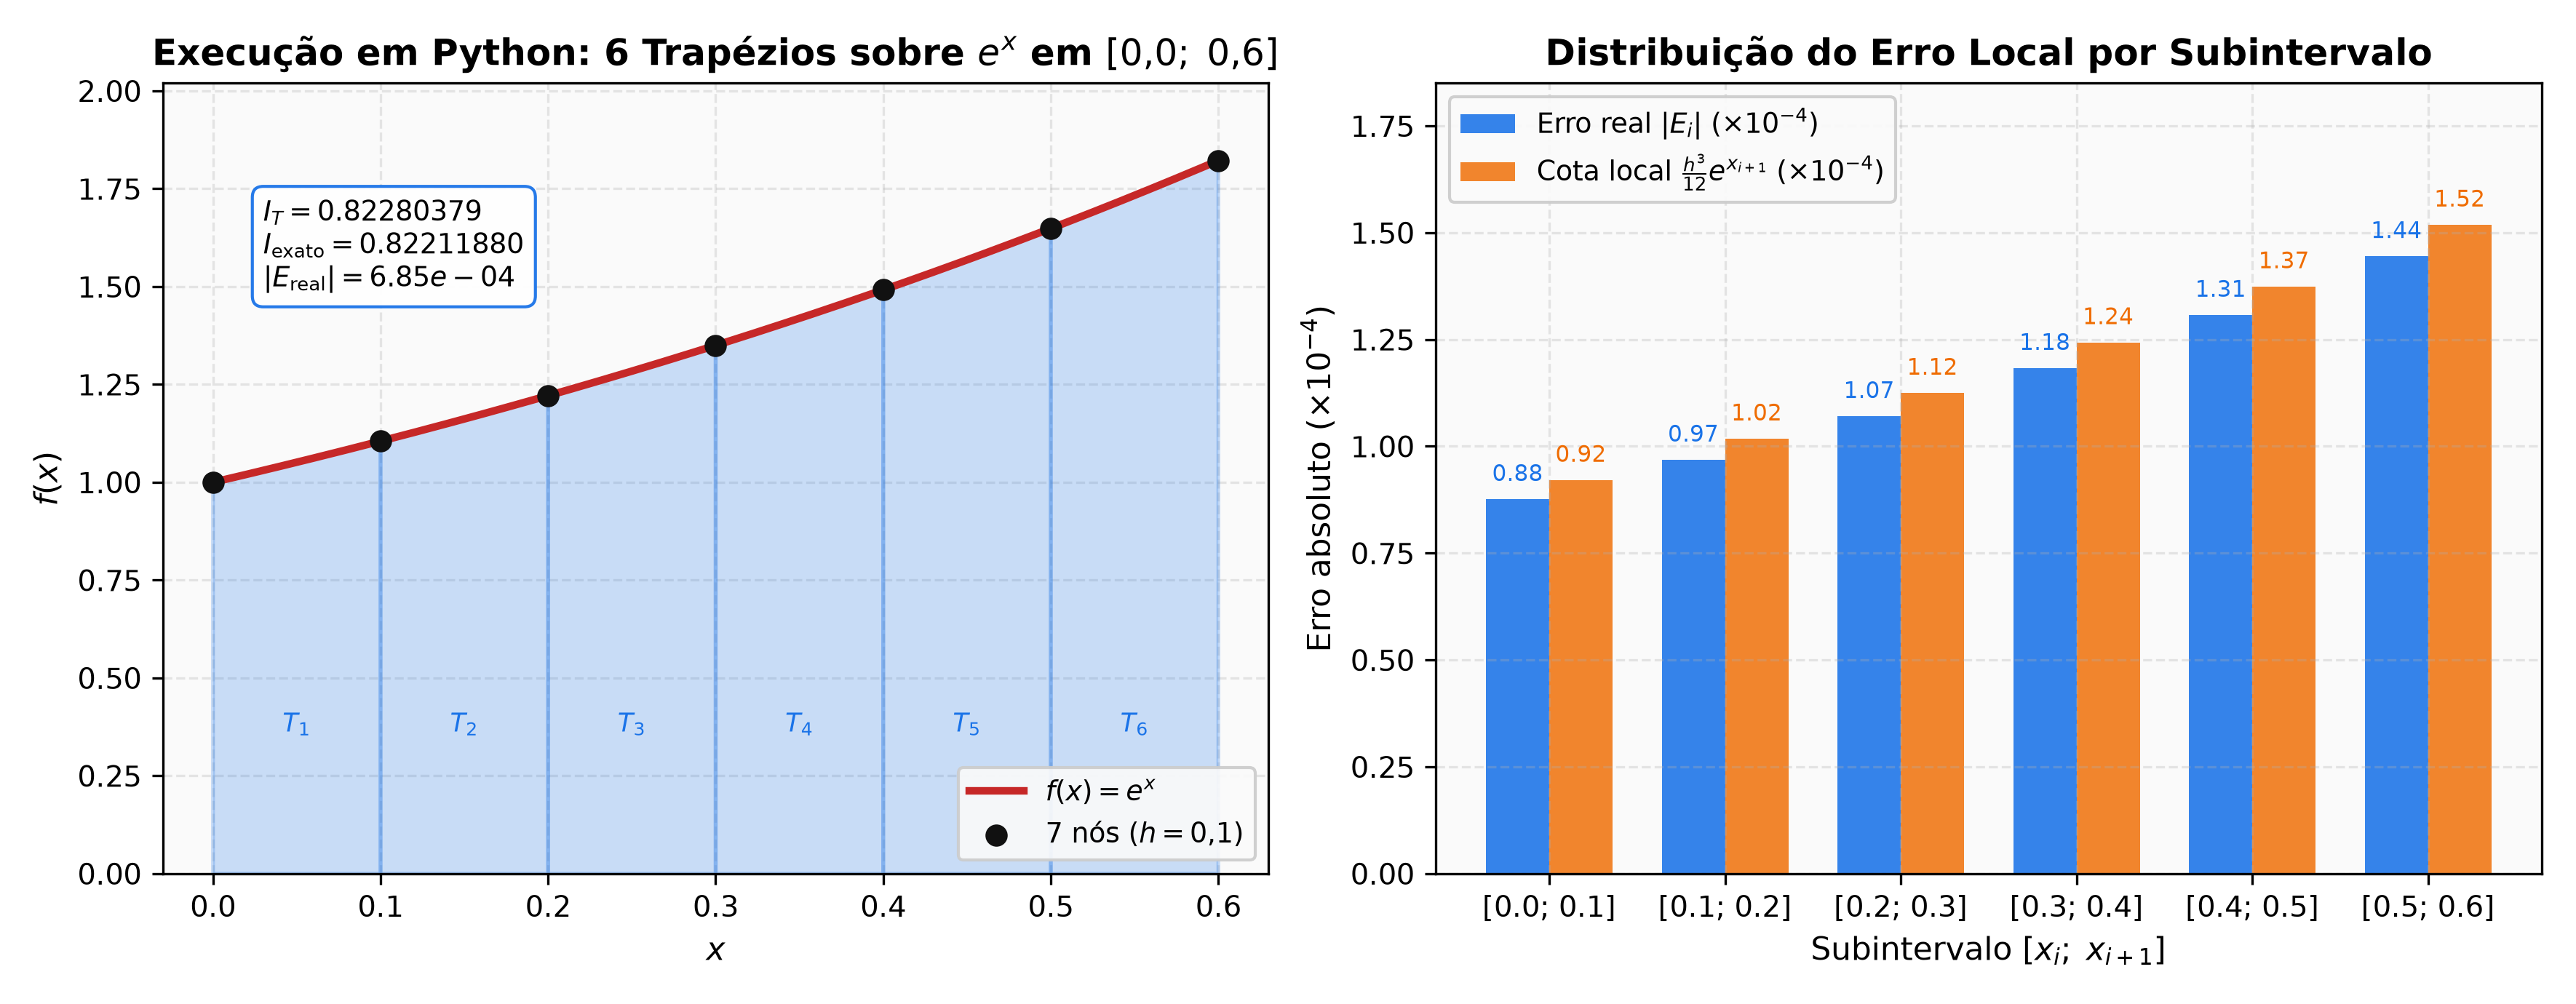
\includegraphics[width=0.95\textwidth]{images/fig_execucao_python_ex.png}
    \caption{Execução computacional do Exercício 1 ($\int_{0,0}^{0,6} e^x\,dx$, $n=6$): (esquerda) construção dos 6 trapézios sobre a curva; (direita) distribuição do erro real local frente à cota teórica em cada subintervalo $[x_i, x_{i+1}]$.}
    \label{fig:exec_python}
\end{figure}

\begin{figure}[h!]
    \centering
    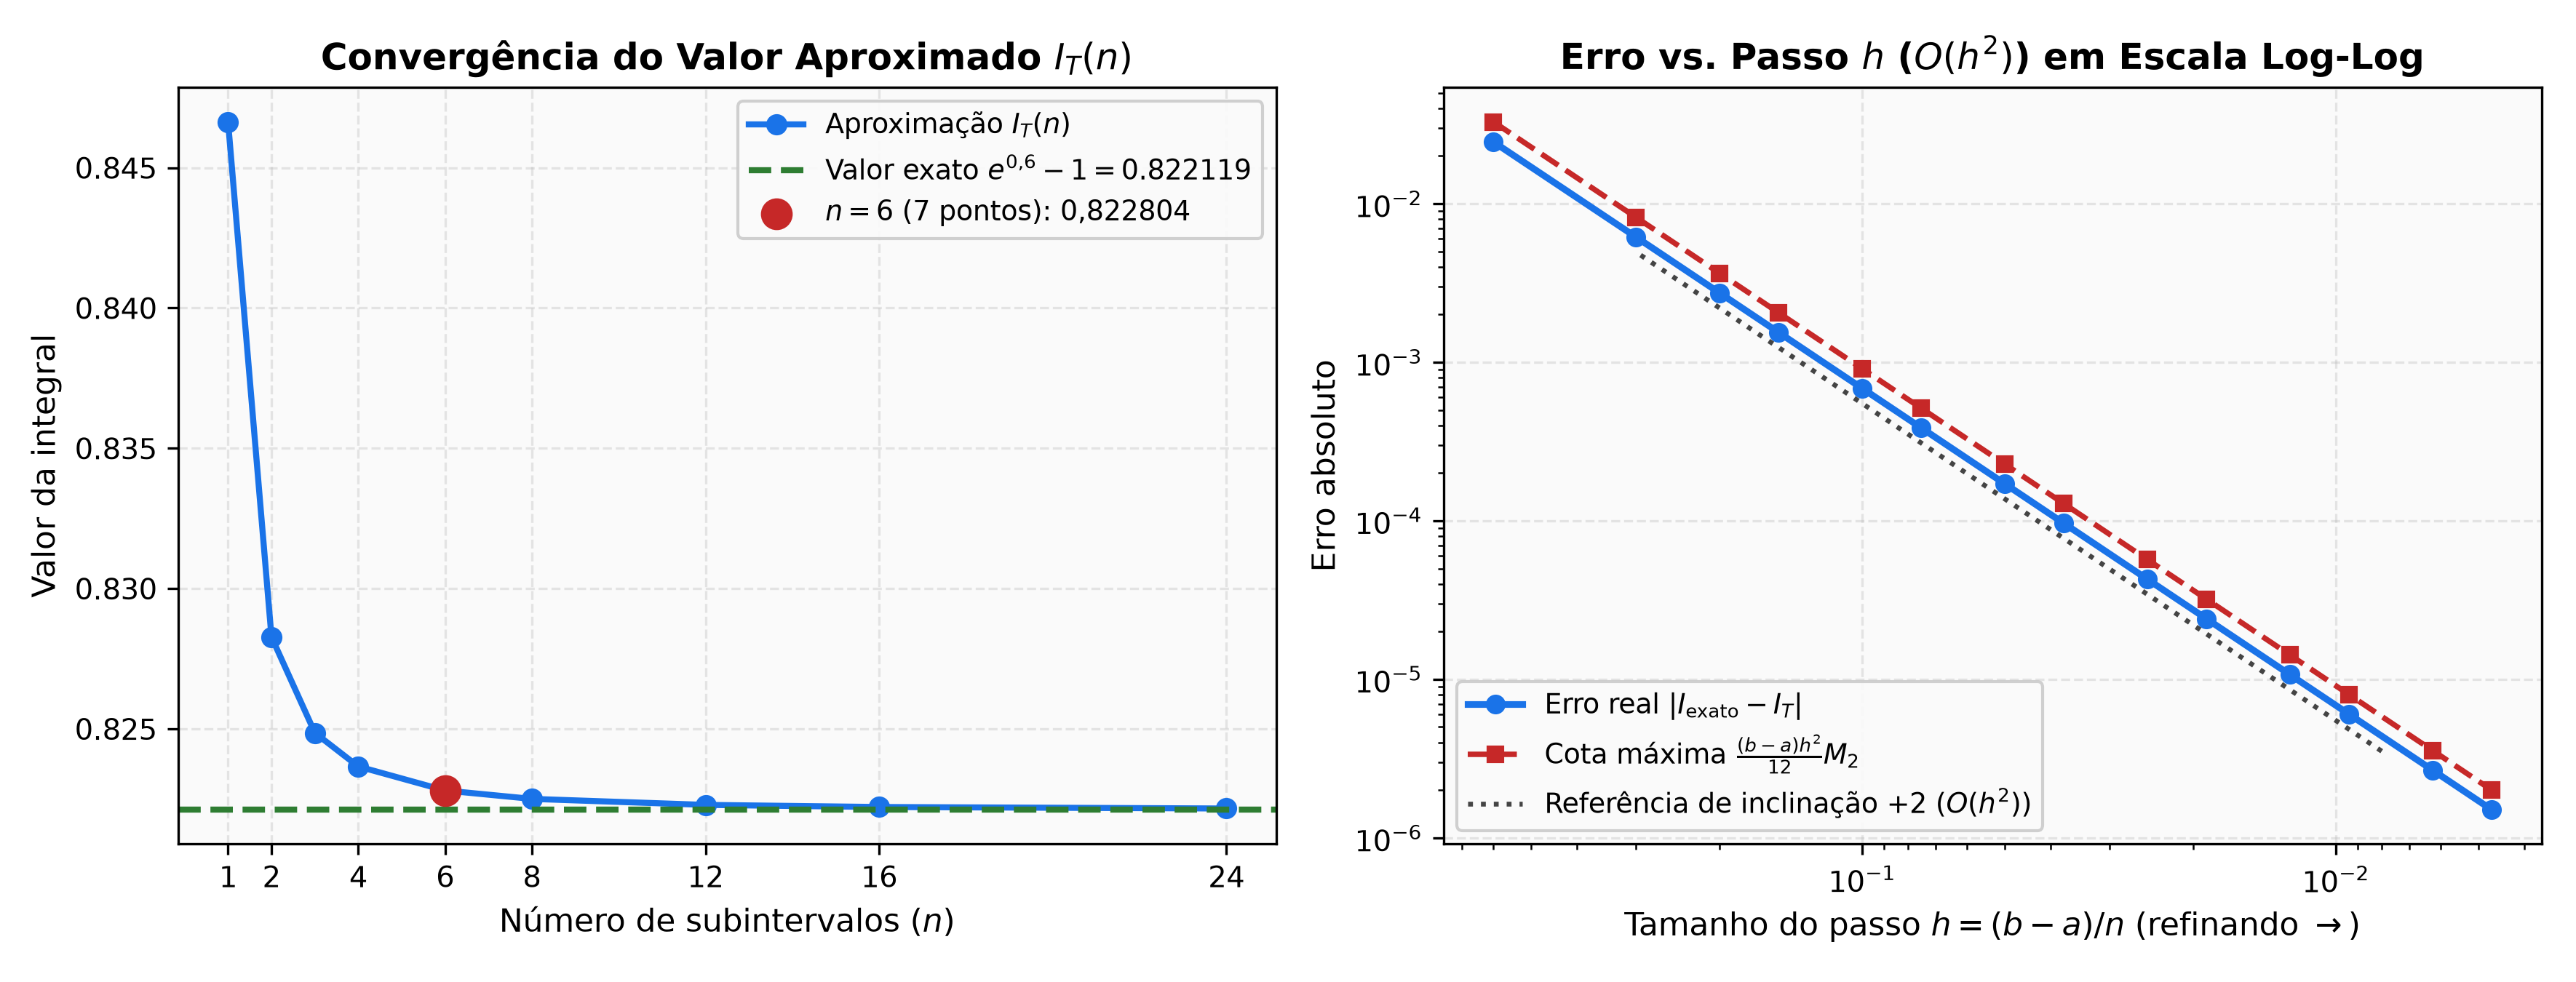
\includegraphics[width=0.95\textwidth]{images/fig_convergencia_erro.png}
    \caption{Estudo assintótico em Python: (esquerda) convergência rápida de $I_T(n)$ ao valor exato; (direita) curva log-log confirmando inclinação exata de ordem $O(h^2)$ para o erro real e para a cota teórica.}
    \label{fig:conv_loglog}
\end{figure}

\begin{figure}[h!]
    \centering
    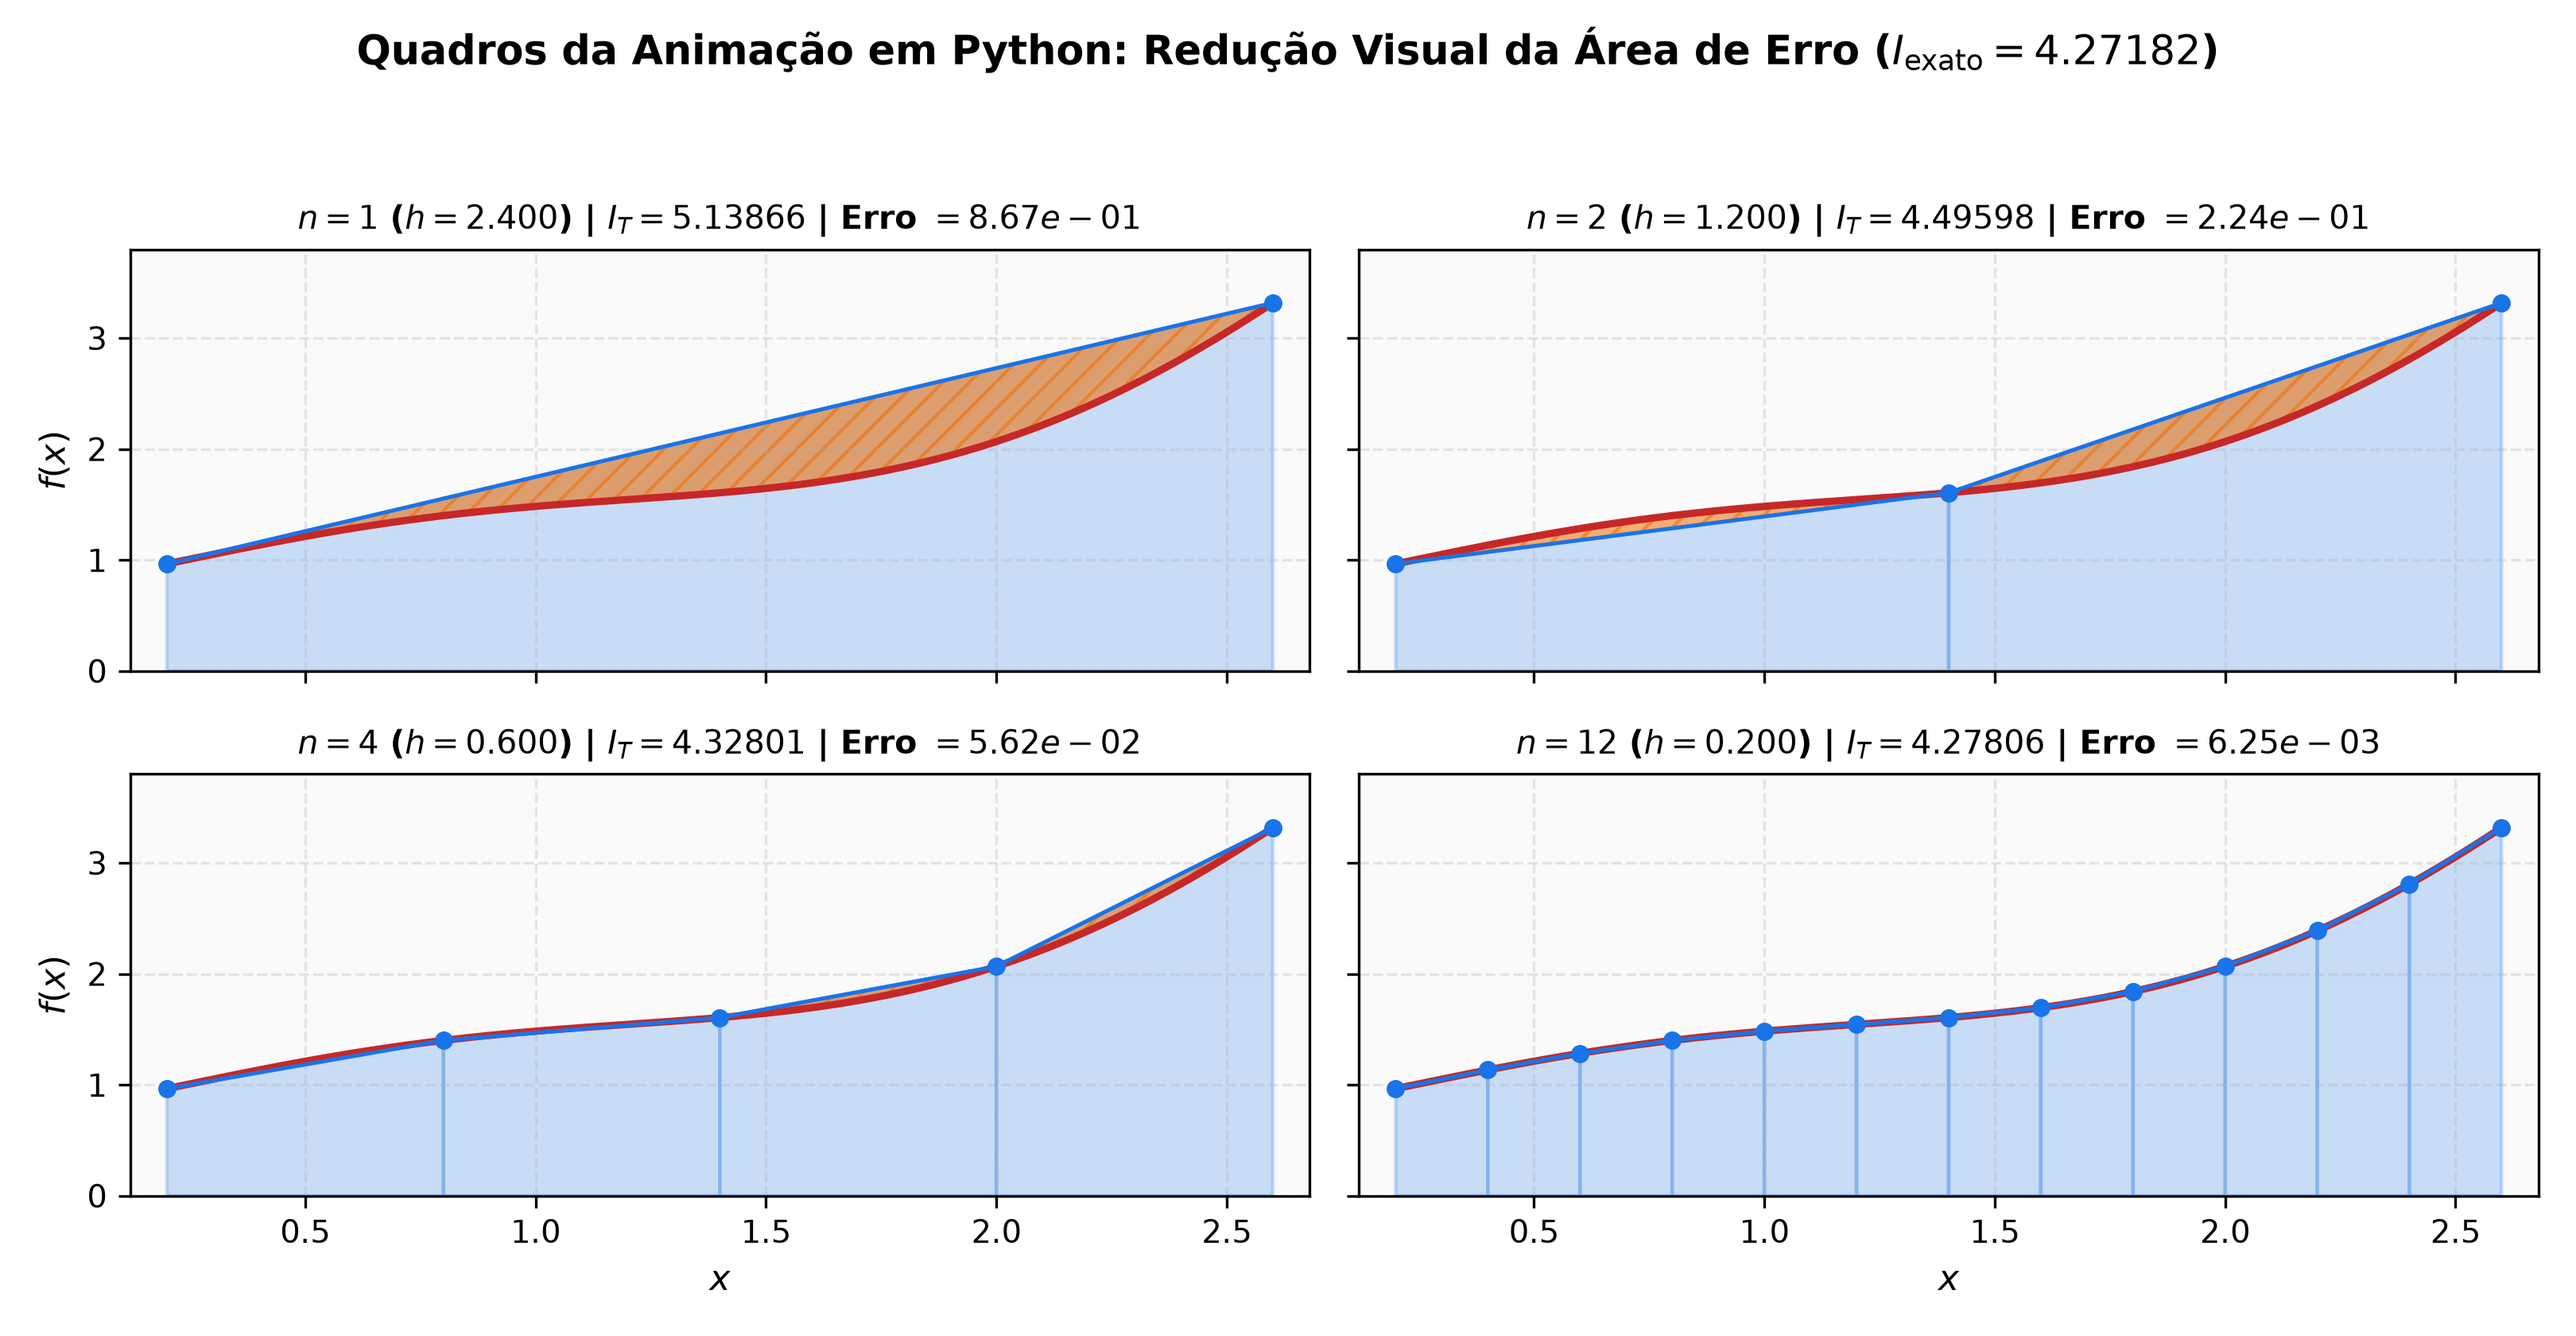
\includegraphics[width=0.92\textwidth]{images/fig_animacao_frames.png}
    \caption{Mosaico com quatro quadros-chave da animação em vídeo (\texttt{videos/animacao\_trapezios.mp4} e \texttt{.gif}), ilustrando o fechamento progressivo da área de erro residual conforme $n$ aumenta.}
    \label{fig:anim_frames}
\end{figure}

\noindent\textbf{Acesso Direto aos Vídeos Gerados:}
\begin{itemize}[leftmargin=1.5em]
    \item Vídeo MP4 local: \href{run:videos/animacao_trapezios.mp4}{\nolinkurl{videos/animacao_trapezios.mp4}}
    \item Animação GIF local: \href{run:videos/animacao_trapezios.gif}{\nolinkurl{videos/animacao_trapezios.gif}}
    \item Repositório GitHub (código, gráficos e vídeos): \href{https://github.com/Zuluke/numerical-calculus.git}{\nolinkurl{https://github.com/Zuluke/numerical-calculus.git}}
\end{itemize}

% ============================================================
% SEÇÃO 7: TRANSIÇÃO PARA A PRÓXIMA AULA
% ============================================================
\section{Indicação para a Próxima Aula: Método de Simpson ($1/3$ e $3/8$)}

Na próxima aula, avançaremos na família de Newton-Cotes elevando o grau polinomial local para $n = 2$ (\textbf{Regra $1/3$ de Simpson}, que aproxima cada par de subintervalos por uma parábola e exige $n$ par) e $n = 3$ (\textbf{Regra $3/8$ de Simpson}, exigindo $n$ múltiplo de $3$) \cite{santos2010, mesquita2026}. Por simetria algébrica no caso $n=2$, o termo de erro em $h^4 f'''$ anula-se, elevando a precisão para $O(h^4)$:
\[
|T_{\text{Simpson } 1/3}| \le \frac{n h^5}{180} M_4, \qquad |T_{\text{Simpson } 3/8}| \le \frac{n h^5}{80} M_4, \qquad M_4 = \max_{x \in [a, b]} |f^{(4)}(x)|.
\]
No exemplo de referência $\int_{0,0}^{0,6} e^x\,dx$ com $7$ pontos ($n = 6$, $h = 0{,}1$), a cota máxima cai de $9{,}1106 \times 10^{-4}$ (Trapézios) para \textbf{$6{,}0737 \times 10^{-7}$} (Simpson $1/3$) --- uma melhora de \textbf{$1.500\times$} utilizando exatamente os mesmos $7$ pontos.

% ============================================================
% SEÇÃO 8: MATERIAIS EXTRAS, VÍDEOS E REFERÊNCIAS
% ============================================================
\section{Materiais Extras, Vídeoaulas e Hyperlinks Explícitos}

\begin{itemize}[leftmargin=1.4em]\small
    \item \textbf{Repositório GitHub do Curso (Prof. João Cardoso)}: \\
    \href{https://github.com/Zuluke/numerical-calculus.git}{\nolinkurl{https://github.com/Zuluke/numerical-calculus.git}} \cite{cardoso2026_github}
    \item \textbf{Portal de Métodos Numéricos --- CIn/UFPE (Prof. Rafael Mesquita)}: \\
    \href{https://cin.ufpe.br/~rgm/metodosnumericos/}{\nolinkurl{https://cin.ufpe.br/~rgm/metodosnumericos/}} \cite{mesquita2026}
    \item \textbf{Ementa e Referências da Disciplina MS211 --- IMECC/UNICAMP}: \\
    \href{https://disciplinas.ime.unicamp.br/ms211/ementa/}{\nolinkurl{https://disciplinas.ime.unicamp.br/ms211/ementa/}} \cite{unicamp_ms211}
    \item \textbf{Vídeoaula Extra [PT-BR] --- UNIVESP (Integração Numérica e Trapézios)}: \\
    \href{https://www.youtube.com/playlist?list=PLxI8Can9yAHdCutIICyWcGI0s-fbpw3fc}{\nolinkurl{https://www.youtube.com/playlist?list=PLxI8Can9yAHdCutIICyWcGI0s-fbpw3fc}} \cite{univesp_video}
    \item \textbf{Vídeoaula Extra [EN] --- Khan Academy (Trapezoidal Approximation)}: \\
    \href{https://www.youtube.com/watch?v=1p0NHR5w0Lc}{\nolinkurl{https://www.youtube.com/watch?v=1p0NHR5w0Lc}} \cite{khan_trapezoid_video}
    \item \textbf{Documentação Oficial SciPy (\texttt{scipy.integrate.trapezoid})}: \\
    \href{https://docs.scipy.org/doc/scipy/reference/generated/scipy.integrate.trapezoid.html}{\nolinkurl{https://docs.scipy.org/doc/scipy/reference/generated/scipy.integrate.trapezoid.html}} \cite{scipy_trapezoid}
\end{itemize}

\nocite{*}
\printbibliography[title={Referências Bibliográficas}]

\vspace{0.8cm}
\begin{flushright}
\textbf{Prof. João Cardoso} --- Cálculo Numérico
\end{flushright}

\end{document}
